\chapter{CONCEPTION ET MODÉLISATION }

\section{Introduction Partielle}

Dans ce présent chapitre, nous allons procéder à la réalisation des diagrammes UML qui nous permettront de bien comprendre notre système, en plus des diagrammes, nous allons définir le processus de développement utilisé et du langage utilisé pour dégager lesdits diagrammes.
\subsection{Présentation du langage UML}

UML est un langage de modélisation très complet, qui couvre de nombreux aspects du développement des logiciels, comme les exigences, l’architecture, les structures et les comportements \cite{xavier_blanc_uml2}.
UML est un langage de modélisation visuelle à usage général pour les systèmes. Bien qu'UML soit le plus souvent associé à la modélisation de systèmes logiciels orientés objet, son application est beaucoup plus large que cela \cite{jim_arlow_uml}.
UML n'est pas lié à une méthodologie ou à un cycle de vie spécifique. Il peut d'ailleurs être utilisé avec toutes les méthodologies existantes. La méthode UP par exemple utilise UML comme syntaxe de modélisation visuelle sous-jacente. Elle est la méthode préférée pour UML, car elle est la mieux adaptée, mais UML fournit le support de modélisation visuelle pour d'autres méthodes \cite{jim_arlow_uml}.

\subsection{Présentation de la méthode DSDM}
La méthode DSDM, encore appelée Méthode de développement de systèmes dynamiques, est une méthode de gestion de projet de la catégorie des méthodes agiles développée en Grande-Bretagne à partir de 1994.
La méthode DSDM fait référence à un processus organisé et fondé sur le bon sens qui donne la priorité à la mise en œuvre rapide et efficace de projets.  À bien des égards, elle est comparable à XP et à Scrum, mais son principal avantage par rapport à ces deux méthodes est qu'il s'agit de la meilleure méthodologie pour laquelle les délais sont fixes. Au lieu de se concentrer sur les activités des équipes de développement, DSDM met l'accent sur la livraison de la solution.  Cette méthodologie fait le nécessaire pour s'assurer que le sens commercial et la faisabilité de chaque projet ont été établis avant la conception et la mise en œuvre \cite{jason_bennett_agile}.

\begin{figure}[H]
	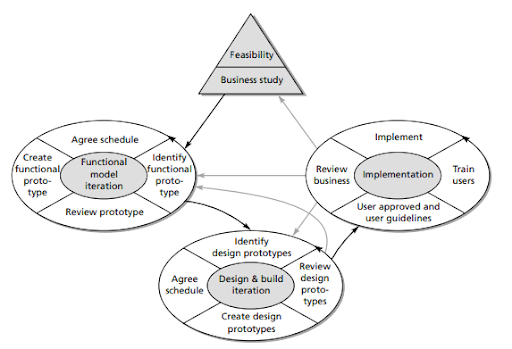
\includegraphics[width=\textwidth]{dsdm}
	\caption{Aperçu général du processus DSDM\cite{the_dsdm_consortium_dsdm}}
\end{figure}


\subsection{Utilisation de l'orienté objet avec le DSDM}
l'analyse orientée objet a commencé par la décomposition du système proposé en cas d'utilisation, qui, pour nos besoins, peuvent être considérés comme des processus métier que le système aidera à résoudre. Cela correspond bien au domaine d'activité de DSDM \cite{the_dsdm_consortium_dsdm}.

\begin{itemize}
	\item Identifier les besoins métier qui devraient être pris en charge par le système proposé.
	\item Définir les besoins en information des processus métier qui seront pris en charge.
	\item Identifier les catégories d'utilisateurs impactés par le développement et l'introduction du système proposé.
	\item Identifier les processus métier et les scénarios métier qui doivent être modifiés.
	\item Clarifier toutes les interfaces avec d'autres systèmes (humains ou automatisés).
	
\end{itemize}

La conception orientée objet consiste essentiellement à sélectionner une architecture (généralement multiniveaux), les protocoles de communication entre les niveaux, une stratégie de gestion au sein des niveaux et les langages appropriés pour construire les niveaux. Encore une fois, cela correspond bien aux objectifs de définition de l'architecture système :

\begin{itemize}
	\item Fournir une compréhension commune des architectures techniques à utiliser pendant le développement et la mise en œuvre.
	\item Décrire la plateforme cible et la plateforme de développement.
	\item Fournir une description générale de l'architecture logicielle (c'est-à-dire les principaux objets ou composants logiciels, à la fois processus et données, et leurs interactions).
\end{itemize}

La technologie orientée objet facilite le développement incrémental du code requis; les concepts d'orientation objet encouragent le développement d'opérations/méthodes de classe petites et réutilisables, qui peuvent être ajoutées au besoin même après que la classe a été déployée \cite{the_dsdm_consortium_dsdm}.


\subsection{Évaluation des risques}
Chaque fonctionnalité d’un logiciel est associée à un risque, qu'il s'agisse d'un risque lié à la disponibilité, à l'évolutivité ou à l'intégrité des données. L'analyse des risques liés à l'architecture est l'une des activités clés de la gestion des projets. En analysant continuellement les risques, l'architecte peut remédier aux lacunes d’un projet et prendre des mesures correctives pour atténuer les risques \cite{mark_richards_fundamentals}.

\section{Besoins}
La conception d’un système exige de connaître les besoins des utilisateurs concernés, voici ci-dessous les besoins que nous avions pu constater; et que nous utiliserons par la suite à des fins de modélisation, enfin de mieux comprendre le système de manière générale.

\subsection{Besoins fonctionnels}
\begin{enumerate}
	\item L’utilisateur doit s’authentifier avant d’accéder à l’application
	\item L’administrateur doit s’authentifier avant d’accéder à l’espace d’administration
	\item L’utilisateur peut ajouter des contacts qui recevront les alertes
	\item L’utilisateur peut consulter la liste de ses contacts.
	\item L’utilisateur peut modifier les contacts qu’il a ajoutés
	\item L’utilisateur peut supprimer des contacts parmi les contacts qu’il a ajoutés
	\item L’utilisateur peut envoyer une alerte
	\item L’administrateur peut consulter les alertes actives de tous les utilisateurs
	\item L’administrateur peut retransmettre les alertes aux contacts de l’utilisateur ou a un centre de sécurité
\end{enumerate}

\subsection{Besoins non fonctionnels}
\begin{enumerate}
	\item l’application doit être intuitive et facile à manipuler
	\item l’application doit être en mesure de fonctionner sur des périphériques non performant 
	\item les informations liées à la géolocalisation des utilisateurs doivent être le plus précises possible
\end{enumerate}

\section{Identification des acteurs}	
\begin{enumerate}
	\item Utilisateur : Une personne qui peut être victime de kidnapping et qui aura besoin d’être assistée
	\item Administrateur : chargé de la gestion du tableau de bord du système
	\item Service de messagerie : un système logiciel externe qui permet d’envoyer des SMS
\end{enumerate}

\section{Diagrammes}
\subsection{Diagramme de cas d’utilisation}
Dans le cadre de notre travail de fin de cycle (TFC), le diagramme de cas d'utilisation revêt une importance cruciale. Il nous sert avant tout à comprendre les besoins et les exigences fonctionnelles du système que nous analysons ou que nous sommes en train de concevoir. En identifiant les acteurs impliqués et en décrivant comment ils interagissent avec le système, ce diagramme nous permet d'établir une base solide pour la planification et la réalisation de notre solution.

\begin{figure}[H]
	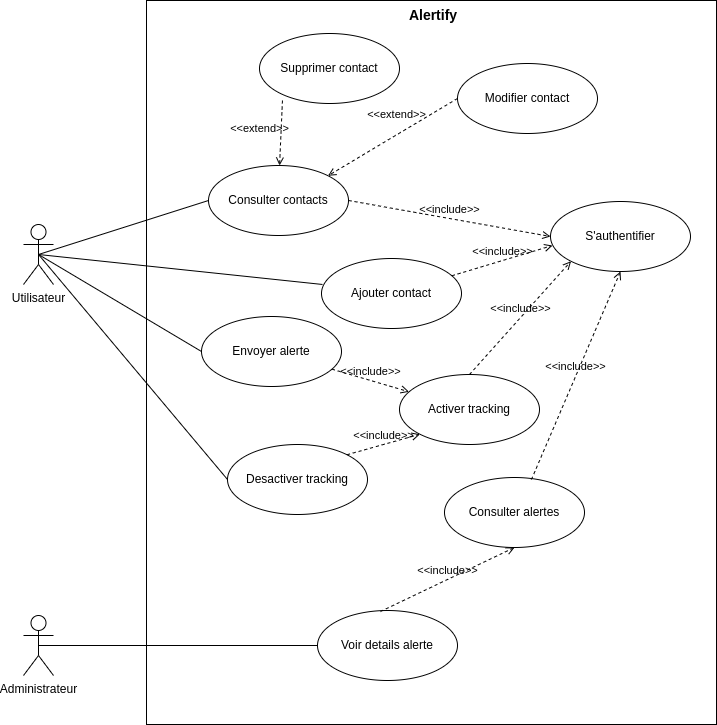
\includegraphics[width=\textwidth]{usecase}
	\caption{Diagramme de cas d’utilisation}
\end{figure}

\subsubsection{Classification des cas d’utilisation}
\begin{table}[H]
	\large
	\captionsetup{justification=raggedright, singlelinecheck=false, font=large,font+=it}
	\caption{Classification des cas d’utilisation}
	\begin{tabularx}{\textwidth}{@{}XXX@{}}
		\hline
		\hline
		\textbf{Cas d’utilisation} & \textbf{Priorité} & \textbf{Risque}\\
		\hline\hline
		S’authentifier & Élevée & Moyen\\
		Consulter contacts & Élevée & Moyen\\
		Ajouter contact & Élevée & Moyen\\
		Modifier contact & Faible & Faible\\
		Supprimer contact & Moyenne & Faible\\
		Activer tracking & Élevée & Moyen\\
		Désactiver tracking & Élevée & Faible\\
		Envoyer alerte & Élevée & Élevée\\
		Consulter alertes & Élevée & Faible\\
		\hline
	\end{tabularx}
\end{table}
\subsubsection{Descriptions textuelles des cas d’utilisation}

\begin{enumerate}[label=\alph*.]
	\item S’authentifier
	\begin{itemize}
		\item Objectif : permettre à l’utilisateur de fournir son identité au système
		\item Acteurs :
		\begin{itemize}
			\item Acteur principal : Utilisateur,Administrateur
			\item Acteur secondaire : -
		\end{itemize}
		\item Précondition : -
		\item Scenario nominal :
		\begin{enumerate}[label=\arabic*.]
			\item L’utilisateur soumet son numéro de téléphone
			\item Le système envoi un code de validation au numéro
			\item Le système affiche le formulaire de soumission du code de confirmation
			\item L’utilisateur soumet le code de confirmation
			\item Le système vérifie la validité du code de confirmation
			\item Le système affiche un formulaire d’insertion d’identité
			\item L’utilisateur soumet son identité
			\item Le système affiche un message de succès 
		\end{enumerate}
		\item Scenario alternatif :
		\begin{enumerate}[label=\arabic*.]
		\item[6] .a. Le code de confirmation est invalide
		\item[6] .a.1. Le système affiche un message d’erreur
		\item[6] .a.2. On rentre au scenario 1
		\end{enumerate}
		\item Scenario d’exception : 
		\begin{enumerate}[label=\arabic*.]
			\item L’utilisateur quitte l’application avant la fin de l’authentification
		\end{enumerate}
		\item Postcondition : L’utilisateur est authentifié et peut accéder aux autres fonctionnalités
	\end{itemize}
	
	\item Consulter contacts
	\begin{itemize}
		\item Objectif : permettre à l’acteur de voir la liste de ses contacts
		\item Acteurs :
		\begin{itemize}
			\item Acteur principal : Utilisateur
			\item Acteur secondaire : -
		\end{itemize}
		\item Précondition : S’authentifier
		\item Scenario nominal :
		\begin{enumerate}[label=\arabic*.]
			\item L’acteur accède à la page des contacts
			\item Le programme affiche la liste de tous ses contacts
		\end{enumerate}
		\item Scenario alternatif : -
	
		\item Scenario d’exception :  -
		\item Postcondition : -
	\end{itemize}
	
	\item Ajouter contact
	\begin{itemize}
		\item Objectif : permettre à l’acteur d’ajouter un contact
		\item Acteurs :
		\begin{itemize}
			\item Acteur principal : Utilisateur
			\item Acteur secondaire : -
		\end{itemize}
		\item Précondition : -
		\item Scenario nominal :
		\begin{enumerate}[label=\arabic*.]
			\item L’utilisateur accède à la page d’ajout de contact
			\item Le formulaire d’ajout est affiché
			\item L’utilisateur soumet le formulaire
			\item Le système vérifie que les informations sont valides
			\item Le système enregistre le contact
			\item Le système affiche un message de succès
		\end{enumerate}
		\item Scenario alternatif :
		\begin{enumerate}[label=\arabic*.]
			\item[5] .a. Les informations sont invalides
			\item[5] .a.1. Le système affiche un message d’erreur
			\item[5] .a.2. On rentre au scenario 2
		\end{enumerate}
		\item Scenario d’exception : -
		\item Postcondition : Un nouveau contact est ajouté
	\end{itemize}
	
	\item Modifier contact
	\begin{itemize}
		\item Objectif : permettre à l’utilisateur de modifier un contact
		\item Acteurs :
		\begin{itemize}
			\item Acteur principal : Utilisateur
			\item Acteur secondaire : -
		\end{itemize}
		\item Précondition : Consulter contact
		\item Scenario nominal :
		\begin{enumerate}[label=\arabic*.]
			\item L’utilisateur sélectionne un contact
			\item L’utilisateur sélectionne l’option de modification du contact
			\item Le système affiche le formulaire de modification du contact
			\item L’utilisateur modifie le contact
			\item L’utilisateur soumet le formulaire
			\item Le système vérifie les nouvelles informations
			\item Le système enregistre les modifications du contact
			\item Le système affiche un message de succès
		\end{enumerate}
		\item Scenario alternatif :
		\begin{enumerate}[label=\arabic*.]
			\item[7] .a. Les informations sont invalides
			\item[7] .a.1. Le système affiche un message d’erreur
			\item[7] .a.2. On rentre au scenario 3
		\end{enumerate}
		\item Scenario d’exception : 
		\begin{enumerate}[label=\arabic*.]
			\item L’utilisateur n’a aucun contact
			\item L’utilisateur quitte la page de modification du contact avant de l’avoir soumis
		\end{enumerate}
		\item Postcondition : Un contact a été modifié
	\end{itemize}	
	
	\item Supprimer contact
	\begin{itemize}
		\item Objectif : permettre à l’utilisateur de supprimer un contact
		\item Acteurs :
		\begin{itemize}
			\item Acteur principal : Utilisateur
			\item Acteur secondaire : -
		\end{itemize}
		\item Précondition : Consulter contact
		\item Scenario nominal :
		\begin{enumerate}[label=\arabic*.]
			\item L’utilisateur sélectionne un contact
			\item L’utilisateur sélectionne l’option de suppression
			\item Le système demande à l’utilisateur de confirmer la suppression
			\item L’utilisateur confirme la suppression
			\item Le contact est supprimé
			\item Le système affiche un message de succès
		\end{enumerate}
		\item Scenario alternatif :
		\begin{enumerate}[label=\arabic*.]
			\item[4] .a. L’utilisateur annule la suppression
			\item[4] .a.1. Le système affiche la liste des contacts
		\end{enumerate}
		\item Scenario d’exception : 
		\begin{enumerate}[label=\arabic*.]
			\item L’utilisateur n’a aucun contact
		\end{enumerate}
		\item Postcondition : Un contact a été supprimé
	\end{itemize}
	
	\item Activer tracking
	\begin{itemize}
		\item Objectif : permettre à l’utilisateur d’activer l’écoute de la commande vocale
		\item Acteurs :
		\begin{itemize}
			\item Acteur principal : Utilisateur
			\item Acteur secondaire : -
		\end{itemize}
		\item Précondition : S’authentifier
		\item Scenario nominal :
		\begin{enumerate}[label=\arabic*.]
			\item L’utilisateur clique sur l’option d’activation de tracking
		\end{enumerate}
		\item Scenario alternatif : -
		\item Scenario d’exception : -
		\item Postcondition : Le système est en attente d’une commande vocale
	\end{itemize}
	
	\item Désactiver tracking
	\begin{itemize}
		\item Objectif : permettre à l’acteur d’annuler l’écoute de la commande vocale
		\item Acteurs :
		\begin{itemize}
			\item Acteur principal : Utilisateur
			\item Acteur secondaire : -
		\end{itemize}
		\item Précondition : Activer tracking
		\item Scenario nominal :
		\begin{enumerate}[label=\arabic*.]
			\item L’utilisateur clique sur l’option de désactivation du tracking
		\end{enumerate}
		\item Scenario alternatif : -
		\item Scenario d’exception : -
		\item Postcondition : L’écoute de la commande vocale est désactivée
	\end{itemize}
	
	\item Envoyer alerte
	\begin{itemize}
		\item Objectif : permettre à l’utilisateur d’envoyer une alerte à ses contacts
		\item Acteurs :
		\begin{itemize}
			\item Acteur principal : Utilisateur
			\item Acteur secondaire : Service de messagerie
		\end{itemize}
		\item Précondition : Activer tracking
		\item Scenario nominal :
		\begin{enumerate}[label=\arabic*.]
			\item L’utilisateur énonce une commande vocale
			\item Le système vérifie la validité de la commande
			\item Tant que le tracking est active, Le service de messagerie envoie une alerte aux contacts de l’utilisateur
		\end{enumerate}
		\item Scenario alternatif :
		\begin{enumerate}[label=\arabic*.]
			\item[1] .a. Le système détecte un son suspect
			\item[1] .a.1. On passe au scenario 3
		\end{enumerate}
		\item Scenario d’exception : 
		\begin{enumerate}[label=\arabic*.]
			\item Le Service de messagerie ne fonctionne pas
			\item Fausse alerte
		\end{enumerate}
		\item Postcondition : Alertes envoyées avec succès
	\end{itemize}
	
	\item Consulter alertes
	\begin{itemize}
		\item Objectif : permettre à l’administrateur de voir les alertes envoyées par les utilisateurs
		\item Acteurs :
		\begin{itemize}
			\item Acteur principal : Administrateur
			\item Acteur secondaire : -
		\end{itemize}
		\item Précondition : S’authentifier
		\item Scenario nominal :
		\begin{enumerate}[label=\arabic*.]
			\item L’administrateur demande la page des alertes
			\item Le système affiche la liste de toutes les alertes
		\end{enumerate}
		\item Scenario alternatif : -
		\item Scenario d’exception : -
		\item Postcondition : -
	\end{itemize}
		
	\item Voir détails alerte
	\begin{itemize}
		\item Objectif : permettre à l’administrateur de voir les détails d’une alerte envoyée par les utilisateurs
		\item Acteurs :
		\begin{itemize}
			\item Acteur principal : Administrateur
			\item Acteur secondaire : -
		\end{itemize}
		\item Précondition : Consulter alertes
		\item Scenario nominal :
		\begin{enumerate}[label=\arabic*.]
			\item L’administrateur demande la page des détails d’une alerte
			\item Le système affiche les détails de l’alerte
		\end{enumerate}
		\item Scenario alternatif : -
		\item Scenario d’exception : -
		\item Postcondition : -
	\end{itemize}
\end{enumerate}

\subsection{Diagrammes de séquence}

Dans le cadre de notre travail, le diagramme de séquence nous permet de modéliser les interactions entre les objets ou composants du système, en mettant en évidence la séquence des messages échangés au fil du temps. Ce diagramme est essentiel pour comprendre le comportement dynamique du système, ce qui facilite la conception ainsi que le développement.

\subsubsection{S'authentifier}
\begin{figure}[H]
	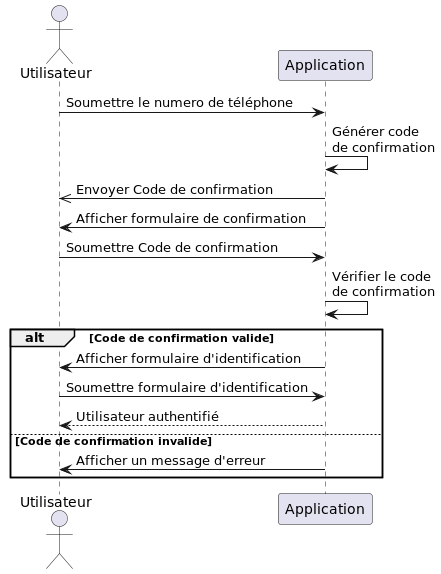
\includegraphics[width=\textwidth]{s_authentifier}
	\caption{Diagramme de séquence S’authentifier}
\end{figure}

\subsubsection{Consulter contacts}
\begin{figure}[H]
	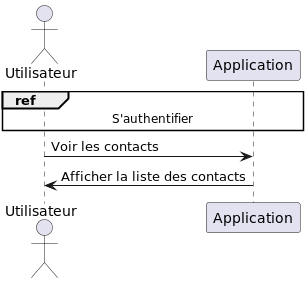
\includegraphics{consulter_contacts}
	\caption{Diagramme de séquence Consulter contacts}
\end{figure}

\subsubsection{Ajouter contact}
\begin{figure}[H]
	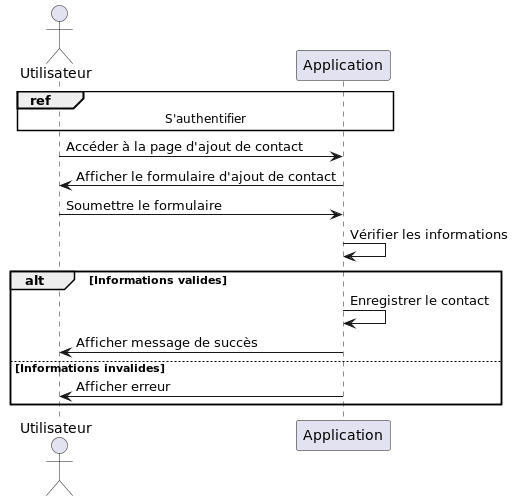
\includegraphics[width=\textwidth]{ajouter_contact.png}
	\caption{Diagramme de séquence Ajouter contact}
\end{figure}

\subsubsection{Supprimer contact}
\begin{figure}[H]
	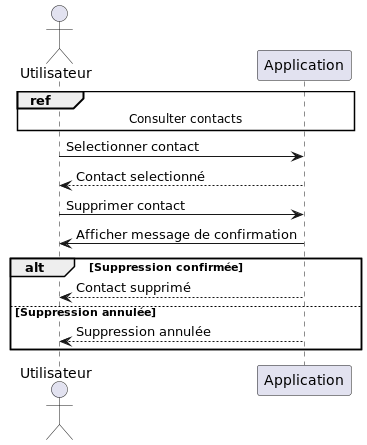
\includegraphics{supprimer_contact}
	\caption{Diagramme de séquence Supprimer contact}
\end{figure}

\subsubsection{Modifier contact}
\begin{figure}[H]
	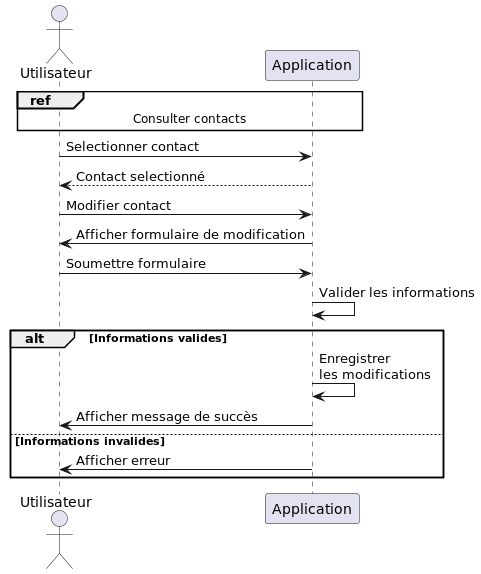
\includegraphics[width=\textwidth]{modifier_contact.png}
	\caption{Diagramme de séquence Modifier contact}
\end{figure}

\subsubsection{Activer tracking}
\begin{figure}[H]
	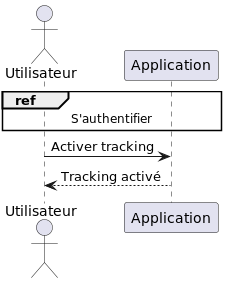
\includegraphics{activer_tracking}
	\caption{Diagramme de séquence Activer tracking}
\end{figure}

\subsubsection{Désactiver tracking}
\begin{figure}[H]
	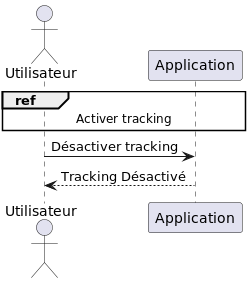
\includegraphics{desactiver_tracking.png}
	\caption{Diagramme de séquence Désactiver tracking}
\end{figure}

\subsubsection{Envoyer alerte}
\begin{figure}[H]
	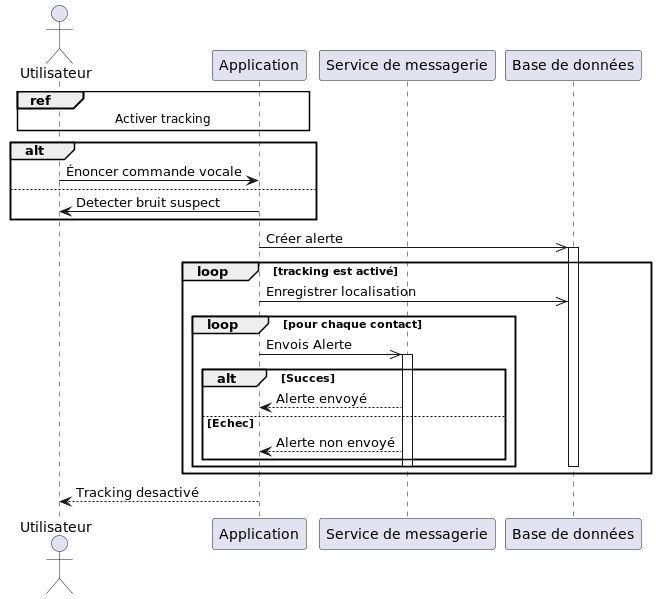
\includegraphics[width=\textwidth]{envoyer_alerte}
	\caption{Diagramme de séquence Envoyer alerte}
\end{figure}

\subsubsection{Consulter alertes}
\begin{figure}[H]
	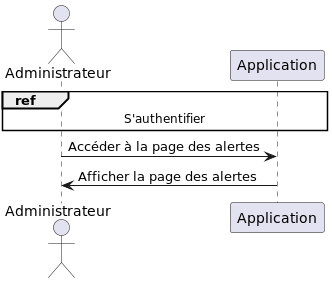
\includegraphics{consulter_alertes}
	\caption{Diagramme de séquence Consulter alertes}
\end{figure}

\subsubsection{Voir détails alertes}
\begin{figure}[H]
	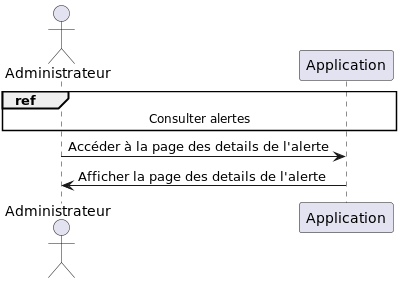
\includegraphics{voir_details_alerte}
	\caption{Diagramme de séquence Voir détails alertes}
\end{figure}

\subsection{Diagramme d’activité}
le diagramme d'activité quant à lui nous permet de modéliser visuellement les processus, les flux de travail, et les décisions au sein du système. En utilisant ce diagramme, nous pouvons mieux comprendre et représenter les séquences d'actions, les transitions, et les conditions qui gouvernent le comportement du système. Cela facilite la planification, la conception et l'optimisation des processus.

\subsubsection{Activité utilisateur}
\begin{figure}[H]
	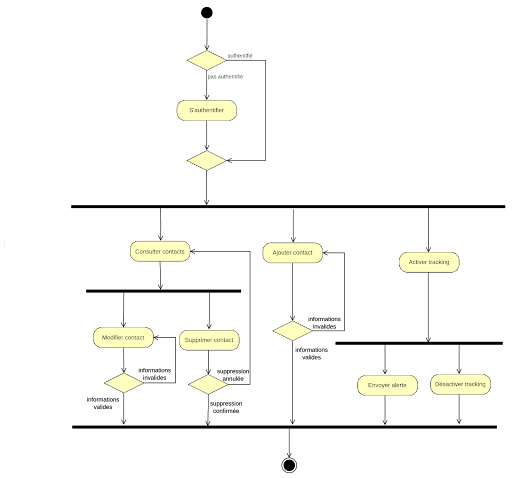
\includegraphics[width=\textwidth]{activity_user}
	\caption{Diagramme de séquence Envoyer alerte}
\end{figure}

\subsubsection{Activité administrateur}
\begin{figure}[H]
	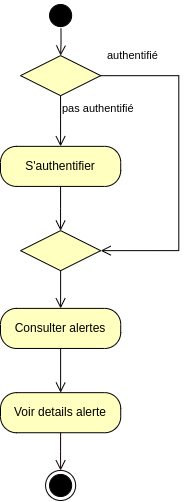
\includegraphics{activity_admin}
	\caption{Diagramme d’activité administrateur}
\end{figure}

\subsubsection{Modèle de domaine}
\begin{figure}[H]
	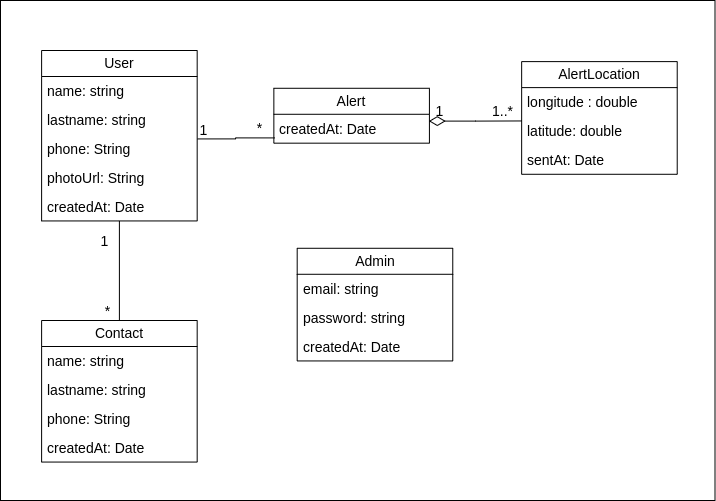
\includegraphics[width=\textwidth]{domain}
	\caption{Modèle de domaine}
\end{figure}

\section{Modélisation de la base de donnes NoSQL orientée document}
La modélisation de la base de données NoSQL constitue une étape cruciale de l'implémentation de notre système. Nous avons opté d’utiliser le service firestore qui propose une base de donnes non relationnelle, sa capacité à gérer efficacement des données géospatiales, sa prise en charge de la synchronisation en temps réel, ainsi que sa scalabilité, en font un choix idéal pour notre application qui nécessite une réactivité immédiate en cas d'urgence.\\

Contrairement aux bases de données relationnelles traditionnelles qui ont une forme simple de disposition en lignes et en colonnes. Une base de données orientée documents stocke les informations au format texte, qui consiste en des collections d'enregistrements organisés selon le concept clé-valeur, c'est-à-dire que pour chaque valeur représentée, un nom (ou étiquette) est attribué, qui décrit sa signification. Ce  modèle de stockage est connu sous le nom d'objet JSON.

\subsection{Règles de mappage pour une base de donnée orientée document}
\subsubsection{Relation par référence}
Ce type de relation stocke les données en incluant des liens ou des références, d'un document à l'autre. Les applications peuvent résoudre ces références pour accéder aux données connexes dans la structure du document lui-même \cite{harley_vera_data}.
\subsubsection{Documents imbriqués}
Ce type de relation est stocké dans une structure de document unique, où les documents imbriqués sont disposés dans un champ ou un tableau. Ces modèles de données dénormalisées permettent de manipuler les données en une seule transaction \cite{harley_vera_data}.

\subsection{Modèle non relationnel}
Voici la manière dont nous avons organisé nos donnes, en priorisant la réduction du nombre de requêtes lors de la lecture.

\begin{figure}[H]
	\centering
	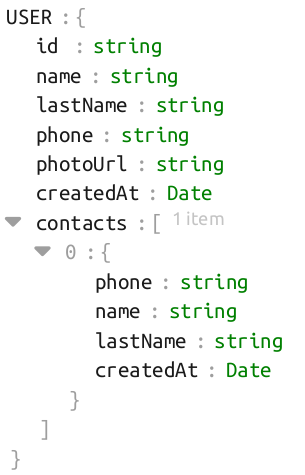
\includegraphics[width=2.23in, height=3.461in,frame]{doc_user}
	\caption{Document utilisateur contenant des sous-documents Contact}
\end{figure}

\begin{figure}[H]
	\centering
	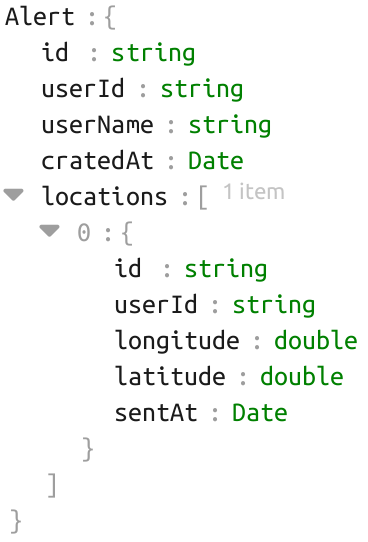
\includegraphics[width=2.23in, height=3.461in,frame]{doc_alert}
	\caption{Document Alert contenant des sous-documents AlertLocation}
\end{figure}

\section{Conclusion partielle}
Pour chaque système d'information, une étape essentielle consiste à le modéliser pour orienter sa concrétisation. Le but de ce chapitre était d'expliquer en détail le fonctionnement du système en utilisant des diagrammes UML. Nous aspirons à atteindre notre objectif, car l'utilisation de multiples diagrammes UML nous a offert une variété de perspectives qui nous seront utiles dans la partie suivante de notre travail, qui sera dédiée à la mise en place de notre solution.

